Negli ultimi decenni il settore delle costruzioni è stato coinvolto nel processo di evoluzione tecnologica.
Questo ha portato ad un cambio di prospettiva e metodologia operativa introducendo il \emph{Building Information Modelling} (BIM).
Esso fornisce un insieme di informazioni geometriche, visive, dimensionali, ambientali, tecniche e operative, rendendo
il processo di progettazione ``sostenibile''.
L'evoluzione è ancora in corso ed il trend è di portare gli applicativi BIM, già presenti nel panorama Desktop, sul Web per renderli
disponibili anche sui dispositivi portatili (smartphone e tablet). L'obiettivo è cercare di portare dei benefici in termini di
disponibilità, affidabilità,
scalabilità, facilità di implementazione, manutenzione e aggiornabilità.

\begin{figure}[htbp] %  figure placement: here, top, bottom, or page
   \centering
   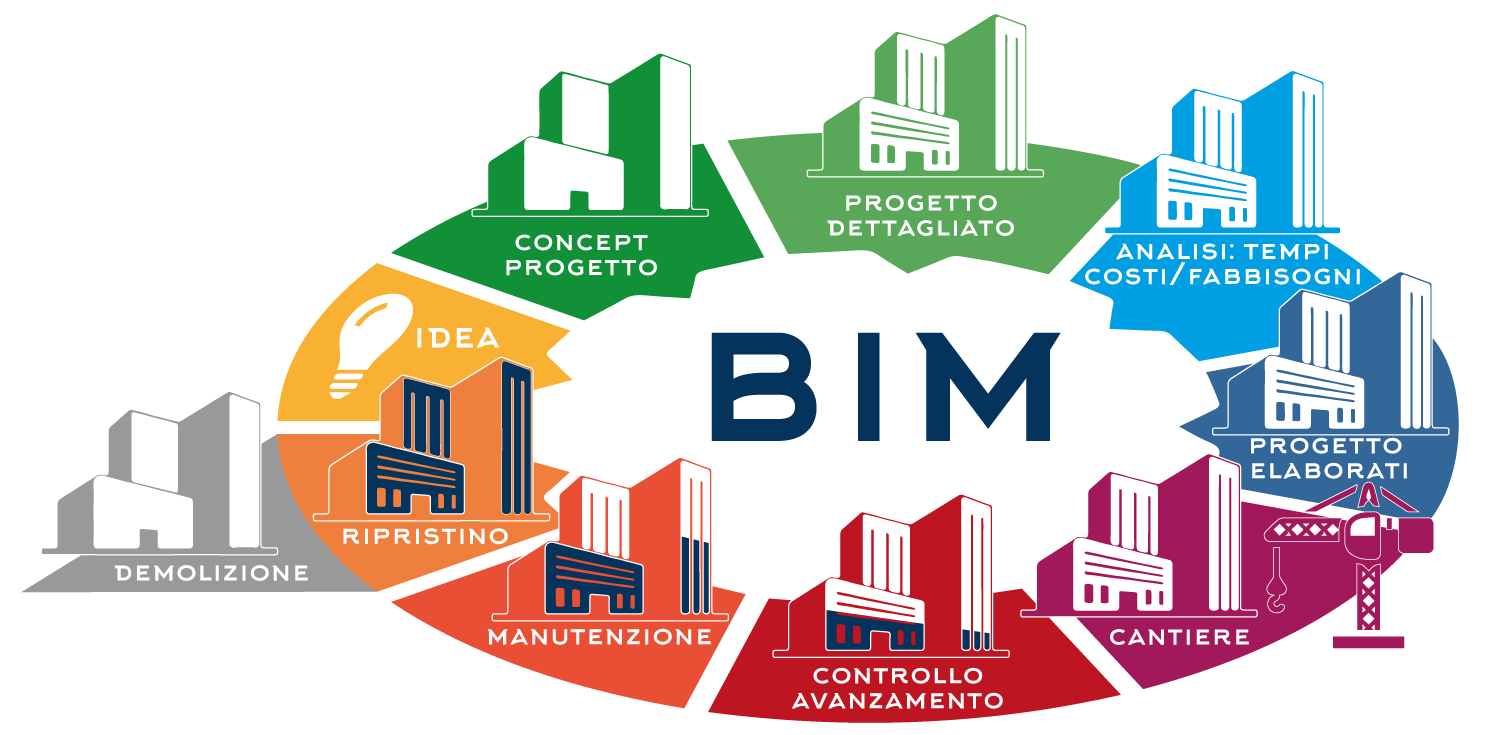
\includegraphics[width=1\linewidth]{images/bim}
   \caption{Fasi coinvolte nel BIM}
   \label{fig:bim}
\end{figure}
\newpage
